\documentclass[beamer,dvipsnames]{standalone}

\usepackage{tikz}
\usetikzlibrary{arrows}
\usetikzlibrary{positioning}
%\usetikzlibrary{positioning,decorations.pathreplacing,fit}
\usetikzlibrary{decorations.markings,arrows.meta,decorations.shapes}

\usepackage{bm}

\providecommand{\adlog}{\textcolor{red}{a}}
\providecommand{\bdlog}{\textcolor{blue}{b}}
\providecommand{\getsr}{\overset{\$}{\gets}}


\definecolor{mygreen}{RGB}{0,128,80}
\colorlet{darkgreen}{mygreen!90!black}

\begin{document}

\begin{standaloneframe}[fragile]

\resizebox{1\textwidth}{!}{

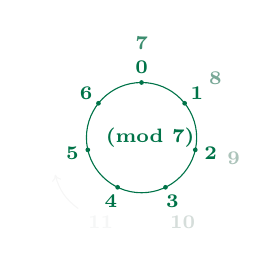
\begin{tikzpicture}[
		every node/.style={
    		font=\bfseries\boldmath,
    		darkgreen
    	},
    	decorate sep/.style 2 args= {decorate,decoration={shape backgrounds,shape=circle,shape size=#1,shape sep=#2}}
	]
	
	
	
	\def\p{7}
	\pgfmathtruncatemacro{\pminus}{\p-1};
	\def\radius{0.7cm}
	

	\coordinate[] (m);

	\draw[thin,darkgreen] (m) circle(\radius) node[align=center] {\scriptsize\hspace*{-3pt}$\pmod 7$};
	
	
	\foreach \s in{0,...,\pminus}{
    	\draw (m)++(-\s*360/\p + 90:\radius) node[fill,circle, inner sep=0.6pt]{};
		\draw (m)++(-\s*360/\p + 90:\radius + 0.2cm) node (p\s) {\scriptsize$\s$};
   	}
   	
   	\foreach \x [count=\s from \p] in {0,1,...,\pminus}{
   		\pgfmathsetmacro{\foo}{max(0,83 - 19*\x)};
		\draw (m)++(-\s*360/\p + 90:\radius + 0.5cm) node (p\s) {\scriptsize$\ifnum\x>6  \else\textcolor{darkgreen!\foo!gray!\foo}{\s}\fi$};
   	}
	
	\draw[-{To[width=1.2mm,length=0.8mm]},thin,gray!7] (p11) to [bend left=19] (p12);
%	\draw[decorate sep={0.8pt}{7pt},fill,lightgray!20] (p11) to [bend left=25] (p12);



	
\end{tikzpicture}

}

\end{standaloneframe}

\end{document}